\chapter{Related Work}
\label{related-work}

None of the qualified teams for the \textit{RoboCup Humanoid League 2019} had a dedicated display
installed on their robots~\cite{robocup-humanoid-teams}. Outside of research contests like
\textit{RoboCup} and industrial applications, user interactions with robots are still rare.
\bigbreak

Relatively common robots for domestic use are automatic vacuum cleaners and lawn mowers. These robots
usually feature only simple displays. Controls are limited to buttons. Complex configuration and
maintenance for most models can be performed using a separate application that has to be installed on
the user's phone. Examples include the \textit{Roomba} and \textit{Braava} product lines by iRobot~\
\cite{irobot-website}.

The \textit{Pepper} robot by SoftBank Robotics is a humanoid robot that focuses on social interactions
in human-centered environments like stores, schools or homes. It is one of the few social robots that
has seen limited success outside of research. In addition to speakers and LEDs it also features a
large touchscreen on the chest. The touchscreen is intended for interaction but can also be used for
debugging during development~\cite{pepper-robot}.

\begin{figure}[h]
      \centering
      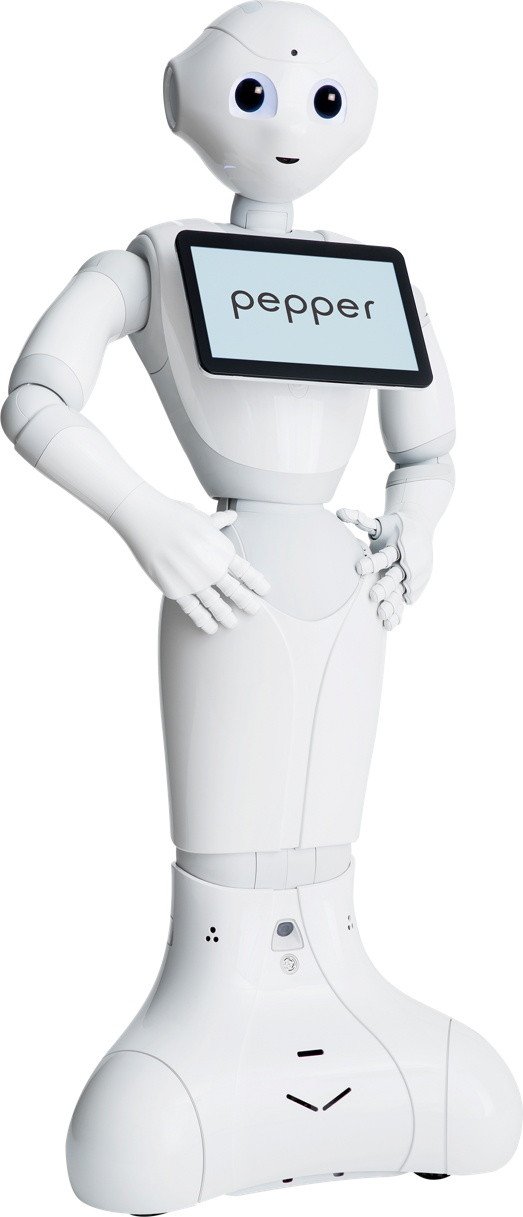
\includegraphics[scale=0.18]{img/pepper.png}
      \caption[The \textit{Pepper} robot]{
          The \textit{Pepper} robot\footnotemark
      }
\end{figure}
\footnotetext{
      Source:~\url{https://www.softbankrobotics.com/emea/themes/custom/softbank/images/full-pepper.png}
      (Accessed: 2020-03-30)
}

Since the \textit{Pepper} robot is highly customizable through software, it can be adapted for a wide
variety of scenarios. However, the lack of powerful or accurate arms limit it to mostly informational
roles. It is used as the platform for the \textit{RoboCup@Home Social Standard Platform League}~\
\cite{pepper-robot}.

Similarly, the \textit{Human Support Robot} by Toyota is used for the \textit{RoboCup@Home Domestic
Standard Platform League}. As the name suggests, these robots are supposed to assist humans in
domestic contexts and are not optimized for complex social interactions. They feature a simple
display for showing additional information~\cite{human-support-robot}.

Many teams in the \textit{RoboCup@Home Open Platform League 2019} also used various types of displays
for interfacing with their robots:

\begin{itemize}
    \item The \textit{CATIE Robotics} team uses modified PAL Robotics \textit{TIAGo} robots. The
          \textit{TIAGo} is equipped with a laptop tray that was customized to make it adjustable.
          An Android tablet was mounted to the back of the head to serve as a touch-capable input
          device~\cite{catie-robotics-tdp}.
    \item The \textit{homer@UniKoblenz} team also uses a \textit{TIAGo} as well as a custom robot based
          on the \textit{CU-2WD-Center} robot platform. It has a small head-mounted display that displays
          a face~\cite{homer-at-uni-koblenz-tdp}.
    \item The \textit{RoboFEI@Home} team uses a custom robot with an enclosure for an Apple iPad \SI{2}{"}
          tablet. The tablet is primarily used to display a face~\cite{robo-fei-at-home-tdp}.
    \item The \textit{RT Lions} team use a screen and a mini-beamer that projects images on a plastic
          dome to display the faces for their two robots~\cite{rt-lions-tdp}.
\end{itemize}
